% Standalone wrapper for paper/figures/hero.tex.
% Build with: latexmk -pdf hero.standalone.tex
% Output:     hero.standalone.pdf  (and .png via pdftoppm)
%
% Mirrors the colour ramps and TikZ libraries from
% paper/style/fair2r.sty so the figure renders identically when
% compiled outside the paper.
\documentclass[tikz,border=4mm]{standalone}

\usepackage[T1]{fontenc}
\usepackage[utf8]{inputenc}
\usepackage{textcomp}
\usepackage{amsmath}        % \text{} inside math mode (used in hero.tex)
\usepackage[scaled=1.0]{helvet}
\renewcommand{\familydefault}{\sfdefault}

\usepackage{xcolor}
\usepackage{tikz}
\usetikzlibrary{arrows.meta, positioning, shapes.geometric}

% --- DLR colour ramps (mirror of paper/style/fair2r.sty) -------------
\definecolor{dlrBlau1}{HTML}{00658B}
\definecolor{dlrBlau5}{HTML}{D1E8FA}
\definecolor{dlrGruen1}{HTML}{82A043}
\definecolor{dlrGruen5}{HTML}{E6EAAF}
\definecolor{dlrGelb1}{HTML}{D2AE3D}
\definecolor{dlrGelb5}{HTML}{FFF8BE}
\definecolor{dlrGrau1}{HTML}{666666}
\definecolor{dlrGrau3}{HTML}{B1B1B1}
\definecolor{dlrGrau4}{HTML}{CFCFCF}
\definecolor{dlrGrau5}{HTML}{EBEBEB}
\colorlet{dlrAccent}{dlrBlau1}
\colorlet{dlrAccentSoft}{dlrBlau5}

\begin{document}
% F(AI)^2R hero figure.
% A horizontal stratification of the writing pipeline: the manuscript
% bundle (the row of named artefacts in the middle, on a hairline grey
% strip) is written into by the (AI)_1 authoring pass arching over it
% from above, and read back by the (AI)_2 audit pass arching under it
% from below. The two arches frame the manuscript as the *shared
% substrate* between writer and reader, which is the central claim of
% the paper: in F(AI)^2R the writing process is itself the artefact
% under audit. Loaded by paper/main.tex (front matter, after \maketitle)
% and referenced from sections/intro.tex.
%
% Self-contained TikZ. A sibling hero.standalone.tex exposes the same
% picture as a standalone document for export to PDF/PNG.
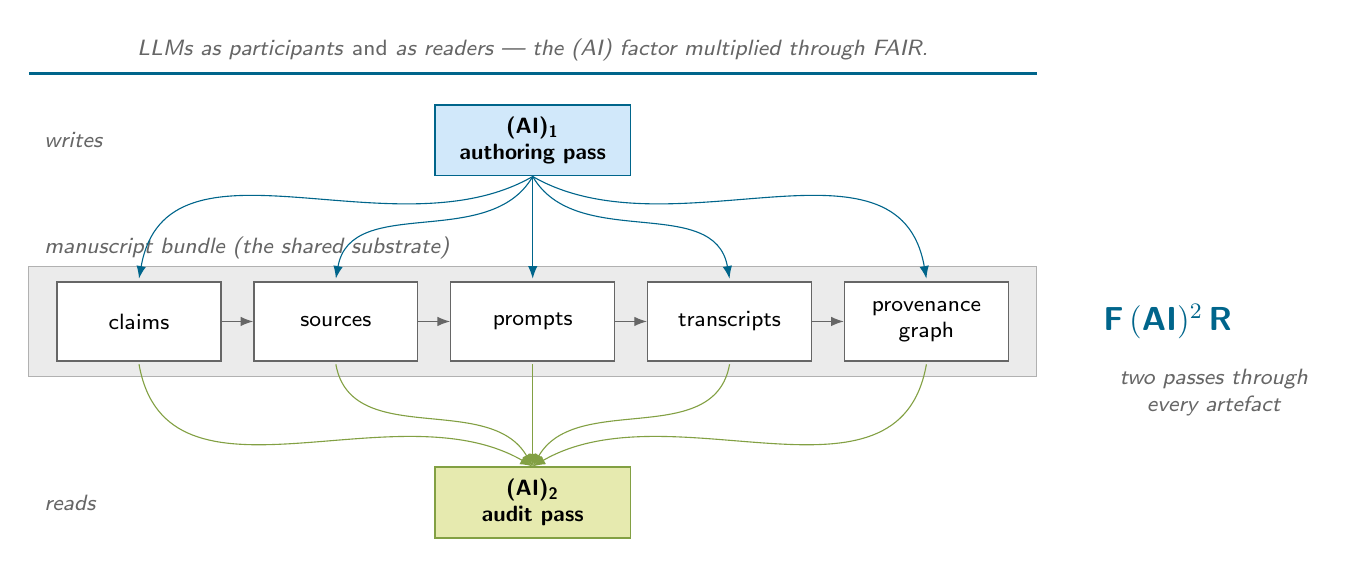
\begin{tikzpicture}[
  every node/.style={font=\sffamily\footnotesize, align=center,
                     inner sep=4pt},
  artefact/.style={draw, line width=0.5pt, draw=dlrGrau1,
                   fill=white, text=black,
                   minimum width=20mm, minimum height=10mm,
                   text width=18mm, align=center},
  authoring/.style={draw, line width=0.5pt, draw=dlrBlau1,
                    fill=dlrBlau5, text=black,
                    minimum width=24mm, minimum height=9mm,
                    text width=22mm, align=center,
                    font=\sffamily\bfseries\footnotesize},
  audit/.style={draw, line width=0.5pt, draw=dlrGruen1,
                fill=dlrGruen5, text=black,
                minimum width=24mm, minimum height=9mm,
                text width=22mm, align=center,
                font=\sffamily\bfseries\footnotesize},
  arrow/.style={-{Latex[length=1.6mm]}, draw=dlrGrau1, line width=0.4pt},
  thickarrow/.style={-{Latex[length=2.0mm]}, line width=0.7pt},
  label/.style={font=\sffamily\itshape\footnotesize, text=dlrGrau1},
]
% --- Middle row: the manuscript bundle as a shared substrate -------
% A hairline grey strip behind the artefact tiles signals "manuscript
% layer". Five tiles correspond to the artefact classes the paper
% argues are produced by LLM-assisted writing.
\fill[dlrGrau5] (-6.4, -0.7) rectangle (6.4, 0.7);
\draw[draw=dlrGrau3, line width=0.3pt]
  (-6.4, -0.7) rectangle (6.4, 0.7);
\node[label, anchor=west, text=dlrGrau1]
  at (-6.35, 0.93) {manuscript bundle (the shared substrate)};

\node[artefact] (claims)      at (-5.0, 0)  {claims};
\node[artefact] (sources)     at (-2.5, 0)  {sources};
\node[artefact] (prompts)     at ( 0.0, 0)  {prompts};
\node[artefact] (transcripts) at ( 2.5, 0)  {transcripts};
\node[artefact] (graph)       at ( 5.0, 0)  {provenance\\graph};

% Hairline connecting the artefacts left-to-right (reading order).
\draw[arrow] (claims.east)      -- (sources.west);
\draw[arrow] (sources.east)     -- (prompts.west);
\draw[arrow] (prompts.east)     -- (transcripts.west);
\draw[arrow] (transcripts.east) -- (graph.west);

% --- Top arch: (AI)_1 authoring pass --------------------------------
\node[authoring] (ai1) at (0, 2.3) {(AI)\textsubscript{1}\\authoring pass};

% Curved arrows from (AI)_1 down to each artefact: writes into them.
\draw[arrow, draw=dlrBlau1]
  (ai1.south) to[out=-150, in=80] ([yshift=1pt]claims.north);
\draw[arrow, draw=dlrBlau1]
  (ai1.south) to[out=-120, in=80] ([yshift=1pt]sources.north);
\draw[arrow, draw=dlrBlau1]
  (ai1.south) -- ([yshift=1pt]prompts.north);
\draw[arrow, draw=dlrBlau1]
  (ai1.south) to[out=-60, in=100] ([yshift=1pt]transcripts.north);
\draw[arrow, draw=dlrBlau1]
  (ai1.south) to[out=-30, in=100] ([yshift=1pt]graph.north);

\node[label, anchor=west] at (-6.35, 2.3)
  {writes};

% --- Bottom arch: (AI)_2 audit pass ---------------------------------
\node[audit] (ai2) at (0, -2.3) {(AI)\textsubscript{2}\\audit pass};

% Curved arrows from each artefact down to (AI)_2: reads them.
\draw[arrow, draw=dlrGruen1]
  ([yshift=-1pt]claims.south)      to[out=-80, in=150] (ai2.north);
\draw[arrow, draw=dlrGruen1]
  ([yshift=-1pt]sources.south)     to[out=-80, in=120] (ai2.north);
\draw[arrow, draw=dlrGruen1]
  ([yshift=-1pt]prompts.south)     -- (ai2.north);
\draw[arrow, draw=dlrGruen1]
  ([yshift=-1pt]transcripts.south) to[out=-100, in=60]  (ai2.north);
\draw[arrow, draw=dlrGruen1]
  ([yshift=-1pt]graph.south)       to[out=-100, in=30]  (ai2.north);

\node[label, anchor=west] at (-6.35, -2.3)
  {reads};

% --- Right-edge synthesis: the "factor multiplied through" -----------
\node[font=\sffamily\bfseries\large, text=dlrAccent, anchor=west]
  at (7.1, 0)  {$\text{F}\,(\text{AI})^{2}\,\text{R}$};
\node[label, text=dlrGrau1, anchor=west, text width=28mm]
  at (7.1, -0.9)  {two passes through every artefact};

% --- Top-edge tagline ------------------------------------------------
\node[font=\sffamily\itshape\footnotesize, text=dlrGrau1]
  at (0, 3.45)
  {LLMs as participants \emph{and} as readers --- the (AI) factor multiplied through FAIR.};
\draw[draw=dlrAccent, line width=0.8pt]
  (-6.4, 3.15) -- (6.4, 3.15);
\end{tikzpicture}

\end{document}
